\documentclass[twoside,11pt]{starlink}

% ? Specify used packages
% ? End of specify used packages



% -----------------------------------------------------------------------------
% ? Document identification
% Fixed part
\stardoccategory    {Starlink User Note}
\stardocinitials    {SUN}
\stardocsource      {sun\stardocnumber}

% Variable part - replace [xxx] as appropriate.
\stardocnumber      {107.4}
\stardocauthors     {M J Bly}
\stardocdate        {6 August 1998}
\stardoctitle     {MAPLE \\[2ex]
                                Mathematical Manipulation Language}
\stardocversion     {Maple V release 4}
\stardocmanual      {User's Guide}
\stardocabstract  {%
MAPLE is a commercial software package for symbolic mathematical
calculation developed by the Symbolic Computation Group at the
University of Waterloo.  Starlink has a licence to run MAPLE on the
central Unix service at RAL. MAPLE has facilities for symbolic algebra
mathematical manipulation and provides a powerful facility for solving
many types of mathematical problem.
}
% ? End of document identification
% -----------------------------------------------------------------------------
% ? Document-specific \providecommand or \newenvironment commands.
% ? End of document-specific commands
% -----------------------------------------------------------------------------
%  Title Page.
%  ===========
\begin{document}
\scfrontmatter

% ? Main text

\section{Introduction\xlabel{introduction}}

MAPLE is an interactive system for symbolic algebra computation. It can
perform hundreds of algebraic functions for use at all mathematical
levels, and can provide solutions for many types of problems:

\begin{itemize}
\item Arithmetic with integers, fractions, and polynomials.
\item Power series.
\item Differentiation and integration of functions.
\item Systems of equations.
\item Differential equations.
\item Linear optimization.
\item Tensor manipulation.
\item Symbolic and numeric approximation.
\item Automatic generation of Fortran code and \LaTeX\ source for mathematical
expressions.
\end{itemize}

In addition, plots can be generated to illustrate graphically any
function, including user-defined functions.

You can extend or redefine the numerous functions by writing MAPLE
programs in the built-in Pascal-like language to create specialized
functions.

\section{\xlabel{using_maple_on_the central_unix_service}
Using MAPLE on the Central Unix Service}

\subsection{\xlabel{registration}Registration}

To use MAPLE you need a user account on the Starlink Central Unix
Service machine at RAL.  Registration is open to Starlink users at UK
Starlink sites.  To obtain an account you should contact the system
manager at RAL by email at \texttt{oper@star.rl.ac.uk}.  When your
application has been processed you will receive an account name and
password (\textit{do not forget to change the password}), and details
of the Central Service machine at RAL.

\subsection{\xlabel{accessing_maple}Accessing MAPLE}

Once you have registered and have logged on to the system at RAL, there
are two versions of MAPLE you can run:

\begin{enumerate}
\item the command-line interface, and
\item the X11 interface.
\end{enumerate}

To start either version you must have \texttt{/usr/local/bin} in your
\texttt{PATH}.  If your login starts the Starlink Software you will get
\texttt{/usr/local/bin} in your \texttt{PATH} automatically.  If your
login does not start the Starlink Software you will need to add
\texttt{/usr/local/bin} to your \texttt{PATH}.

\subsection{\xlabel{the_command-line_interface}The command-line interface}

The command-line interface provides a simple method of using MAPLE which
allows character input and output only with no fancy graphics or animation.
It does provide simple character plots.

To start the command line interface, just type:

\begin{terminalv}
% maple
\end{terminalv}

(\texttt{\%} is the shell prompt).

You will see a banner similar to this:

\begin{terminalv}
% maple
    |\^/|     Maple V Release 4 (WMI Temporary License)
._|\|   |/|_. Copyright (c) 1981-1996 by Waterloo Maple Inc. All rights
 \  MAPLE  /  reserved. Maple and Maple V are registered trademarks of
 <____ ____>  Waterloo Maple Inc.
      |       Type ? for help.
>
\end{terminalv}

(\verb+>+ is the MAPLE command-line prompt).

You can access the help system for MAPLE by using the \texttt{`?'} command.
An introduction is available if you type:

\begin{terminalv}
> ?intro
\end{terminalv}

To leave the MAPLE command-line interface and exit back to the shell,
use the \texttt{`quit'} command:

\begin{terminalv}
> quit
bytes used=374712, alloc=393144, time=0.18
%
\end{terminalv}

\subsection{\xlabel{the_X11_interface}The X11 interface}

The X11 interface is the recommended way to use MAPLE and provides the full
range of facilities.

If you want to use the X11 interface for MAPLE you must first direct
the X output from the RAL machine back to your local system (Xterminal or
system console).

To do this, use the \texttt{xdisplay} command:

\begin{terminalv}
% xdisplay your.machine.name
\end{terminalv}

or set the \texttt{DISPLAY} variable by hand:

\begin{terminalv}
% setenv DISPLAY  your.machine.name:0.0
\end{terminalv}

You should also make sure you have allowed access to the local system by
setting the secuity masks using the \texttt{xhost} command on your local
machine:

\begin{terminalv}
% xhost +central.machine.name
\end{terminalv}

When you have X output directed to your local system you should start the
X11 interface with the \texttt{xmaple} command:

\begin{terminalv}
% xmaple
\end{terminalv}

A window similar to Figure~\ref{fig_main_window} will be generated on your
console/Xterminal.

\begin{figure}[h]
\begin{center}
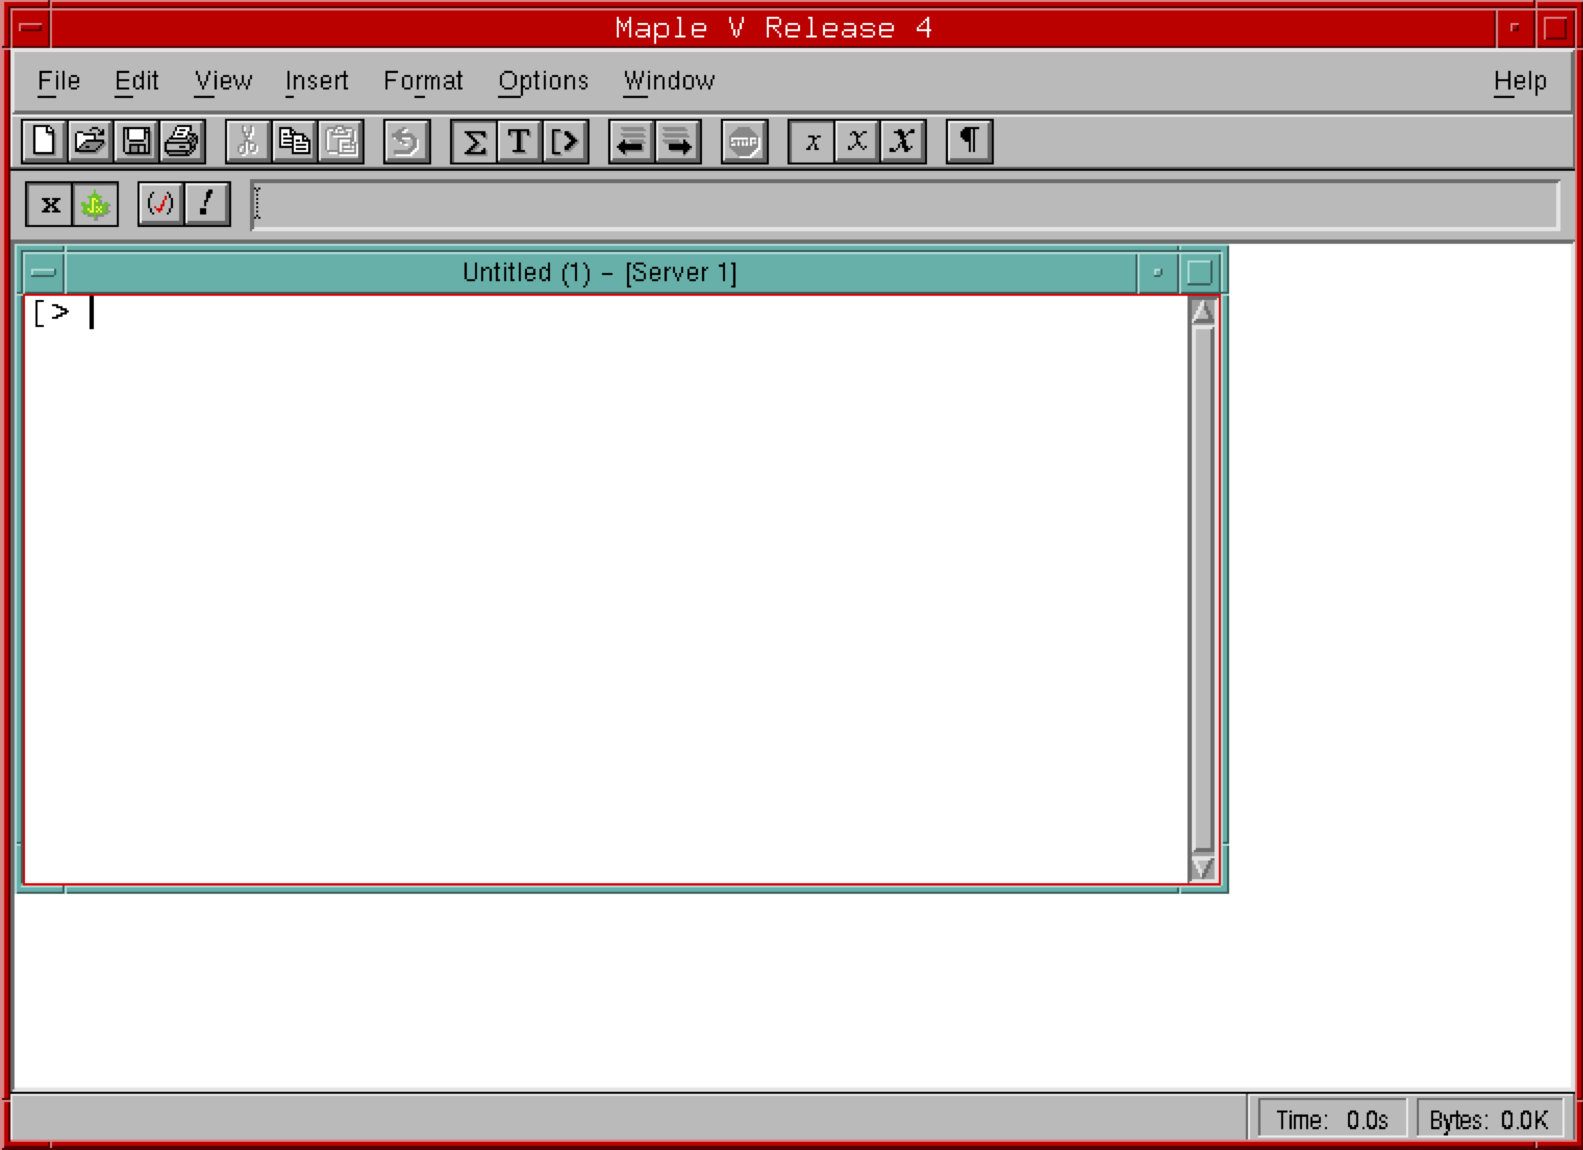
\includegraphics[scale=0.55]{sun107_f1}
\caption{The MAPLE X interface main window}
\label{fig_main_window}
\end{center}
\end{figure}

To quit the X11 interface you should use the \textbf{Exit} button on the
pull-down \textbf{File} menu in the top left corner of the main window.

\section{Examples\xlabel{examples}}

The following example of a MAPLE session should give you some insight
into the capabilities of the software, and how to use it.  You type the
lines after the \verb+>+ prompt and the computer replies with the next line.
The notes after the example explain some of the features you may find
mysterious at first reading.

\begin{terminalv}
> 3+4+5;
                               12
> e1:=expand(x*(x+1)*(x-1));
                               3
                        e1 := x  - x
> factor(");
                        x (x + 1) (x - 1)
> evalf(sqrt(2));
                        1.414213562
> solve(e1=0,x);
                        0, 1, -1
> int(x*exp(x),x);
                        x exp(x) - exp(x)
> help(plot);
     ... gives information on the plot command
> help(index,library);
     ... lists the functions in the Maple library
> quit
     ... escapes from Maple
\end{terminalv}

The second command illustrates the assignment operator \texttt{`:='}. It
assigns the expression on the right of the operator to the variable
(\texttt{e1}) on the left.

The \texttt{(")} symbol refers to the previous expression in the MAPLE
session. Thus the third command \texttt{factor(")} is equivalent to
\texttt{factor(e1)}. There are also symbols \texttt{("")} and \texttt{(""")}
which refer to the second previous and third previous expressions.

In the fifth command, the symbol \texttt{`e1'} refers to the expression
defined in the second command. The \texttt{`int'} function integrates the
expression \texttt{`e1'} with respect to \texttt{x}.

Many examples of how to use MAPLE are given in the on-line help text.
Other examples are stored in files in the \texttt{/usr/local/maple/examples}
directory.

\section{Functions\xlabel{functions}}

MAPLE has a very large number of functions available. You can find an
explanation of these functions and examples of their use by typing the
command:

\begin{terminalv}
> help(<function>);
\end{terminalv}

during a MAPLE session. For example,

\begin{terminalv}
> help(int);
\end{terminalv}

will describe the \texttt{`int'} function which performs integration.

Among the most important and commonly used functions are the following:

\begin{quote}
\begin{description}

\item [expand, simplify, normal] -- simplify expressions.
\item [evalf] -- evaluate an expression using floating point arithmetic.
\item [solve] -- solve equations.
\item [int, diff] -- integrate/differentiate expressions.
\item [series] -- expand functions to Taylor or Laurant series.
\item [plot] -- plot functions.

\end{description}
\end{quote}

Use \verb+help(<function>)+ to find out about these -- there are lots of
examples. Other commonly used functions are:

\begin{quote}
\begin{description}

\item [array] -- create an array.
\item [coeff] -- extract a coefficient of a polynomial.
\item [collect] -- collect terms in a specified indeterminate.
\item [convert] -- convert an expression to a different form.
\item [degree] -- determine the highest degree of a polynomial.
\item [evalc] -- evaluate in the complex number field.
\item [ifactor] -- integer factorisation.
\item [limit] -- calculate function limits.
\item [map] -- apply a procedure to each operand of an expression.
\item [op] -- extract operands from an expression.
\item [product] -- product of a sequence.
\item [radsimp] -- simplification of an expression containing radicals.
\item [subs] -- substitute sub-expressions into an expression.
\item [sum] -- definite and indefinite summation.
\item [table] -- create a table with initial values.
\item [type] -- type checking function.

\end{description}
\end{quote}

These are just a sample of the large number of functions in the standard and
miscellaneous MAPLE function library. In addition, there are a number of
packages which specialise in particular areas of mathematics. These are:

\begin{quote}
\begin{description}

\item [combinat] -- combinatorial functions.
\item [difforms] -- differential forms.
\item [geometry] -- Euclidean geometry.
\item [grobner] -- Grobner bases.
\item [group] -- permutation and finitely-presented groups.
\item [linalg] -- linear algebra.
\item [np] -- Newman-Penrose formalism.
\item [numtheory] -- number theory.
\item [orthopoly] -- orthogonal polynomials.
\item [powseries] -- formal power series.
\item [projgeom] -- projective geometry.
\item [simplex] -- linear optimization.
\item [stats] -- statistics.
\item [student] -- student calculus.

\end{description}
\end{quote}

Information on these packages can be obtained from within MAPLE by
entering:

\begin{terminalv}
> help(<package>);
\end{terminalv}

and information on the functions within a package can be obtained by:

\begin{terminalv}
> help(<package>,<topic>);
\end{terminalv}

Thus, if you were learning calculus you could find help by entering:

\begin{terminalv}
> help(student);
\end{terminalv}

and if you were particularly interested in finding out how to integrate
by parts, enter:

\begin{terminalv}
> help(student,intparts);
\end{terminalv}

Sounds a great way of doing your Maths homework.

% ? End of main text
\end{document}

